\documentclass[a4paper,oneside]{memoir}



\usepackage[utf8]{inputenc}
\usepackage{pdfpages}
\usepackage[scaled]{helvet}
\renewcommand*\familydefault{\sfdefault}
\usepackage[T1]{fontenc}
\usepackage{etoolbox,xparse,environ}

% margins
\usepackage[margin=2.25cm]{geometry}

% tables, links etc
\usepackage{tabu,longtable}
\usepackage{hyperref}

% drawings
\usepackage{tikz}
\usetikzlibrary{shapes.misc,shadows}

% Chapter titling
\usepackage{titlesec}
\titleformat{\chapter}[display]
  {\normalfont\bfseries}{}{0pt}{\Huge}
\titleformat{\section}[display]
  {\normalfont\bfseries}{}{0pt}{\Large}
  
  
% misc
\usepackage{lipsum}

% programme
\newif\ifshowProgramme
\showProgrammefalse

\DeclareDocumentCommand{\day}{m}{%
    \hfill\\\textbf{\LARGE{#1}}\hfill%
}


\NewEnviron{sessions}{%
	\begin{longtabu}[t]{@{}lX[5,l,p]@{}}%
		\BODY%
	\end{longtabu}%
}

% \session{time}{name}[chair]
\DeclareDocumentCommand{\session}{m m o}{%
    \begin{tikzpicture}[baseline=(char.base)]%
    \node(char)[draw,fill=white,%
      shape=rounded rectangle,%
      drop shadow={opacity=.1},%
      minimum width=1.8cm]%
      {#1};%
    \end{tikzpicture} & \large{\textbf{#2}} \\%
    \IfValueT{#3}{& \textit{Session chair: #3}\\[.5cm]}%
}

% \event{type}{title}[authors]{id}
\DeclareDocumentCommand{\event}{m m o m}{%
    & \begin{tabu}[t]{@{}X[p]@{}}{#2}\vspace{.15cm} \\ {\itshape #3}\vspace{.25cm}\end{tabu} \\[.25cm]
    %& \begin{tabu}[t]{@{}X[p]@{}}{\itshape #4}\end{tabu} \\[.5cm]
}


% toc
\newif\ifshowToC
\showToCfalse
\NewEnviron{toc}{%
	\begin{longtabu}[t]{@{}lX[5,l,p]@{}}%
		\BODY%
	\end{longtabu}%
}

% \tocpaper[id]{title}{authors}
\DeclareDocumentCommand{\tocpaper}{o m m}{%
    #1 & \begin{tabu}[t]{@{}X[p]@{}}{#2}\vspace{.15cm} \\ {\itshape #3}\vspace{.25cm}\end{tabu} \\[.25cm]
}


    
\title{Halfway to the Future Programme}
\author{Martin Porcheron}
\date{July 2019}

\begin{document}


\frontmatter
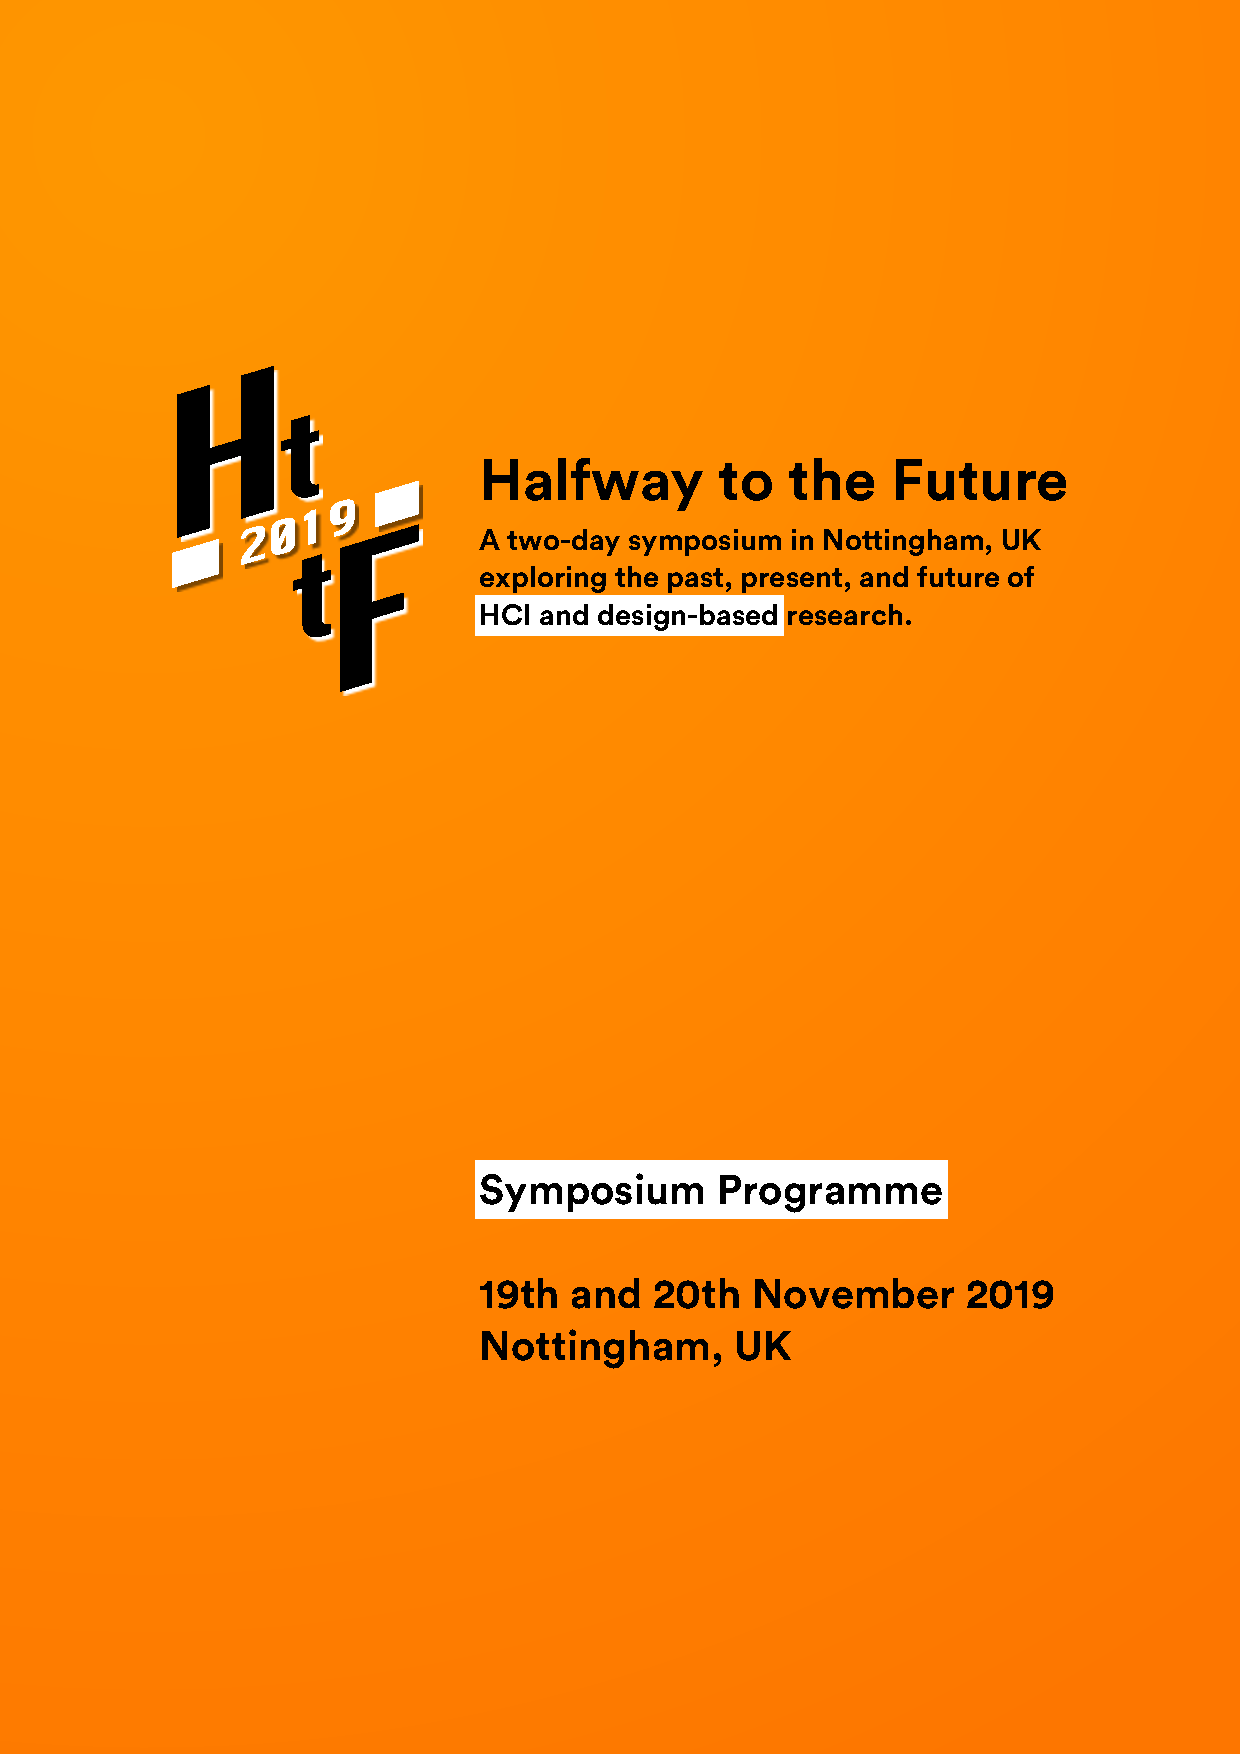
\includepdf[fitpaper=true]{PDFCover.pdf}

\thispagestyle{empty}
\vspace*{\fill}
\begin{raggedright}
    \href{https://www.halfwaytothefuture.org/}{www.halfwaytothefuture.org}\\[.5cm]
    Proceedings of the Halfway to the Future Symposium 2019,\\held at the Albert Hall Conference Centre, Nottingham, UK.\\[.5cm]
    Published by the Association for Computing Machinery, New York, NY, USA.\\
    ISBN-13: 978-1-4503-7203-9\\[.5cm]
    Front matter \textcopyright~University of Nottingham
\end{raggedright}
\clearpage

\mainmatter
\pagestyle{plain}


\chapter{Introduction}
In early 2018, thoughts at the Mixed Reality Laboratory at the University of Nottingham turned to the impending 20\textsuperscript{th} anniversary of the lab's foundation, in 1999. It was suggested by someone---who will remain nameless---that it would be great if we hosted a small `celebration' to mark the occasion. Skip forward in time to November 2019 and we find ourselves hosting an international conference with a full programme featuring 6 keynotes, 42 long and short papers, and a substantial number of attendees. 

How did this happen? Put simply, Halfway to the Future \textit{grew organically}. The logic of symposium had always been to explore the theme of past, present, and future of HCI and design-led research, with a focus on work that we felt had been deeply formative in shaping the research culture of the Mixed Reality Lab throughout its 20 year existence. It was on this basis that we selected themes and keynotes.

%\section{Themes and keynotes}
As we began to reflect upon the past 20 years, 6 themes emerged. These themes were then anchored around a particular piece of highly influential work. These all turned out to be very broad and formed the basis of 6 sessions. Unlike a typical conference with one or two keynote speakers that are kept separate from the main proceedings, we wanted each session to mix keynotes with peer reviewed long and short papers, and to bring together all participants in each panel to conclude with a discussion. Our six themes were:

\begin{itemize}
    \item \textbf{Mixed Reality} with a keynote by Steve Benford, reflecting on the paper \textit{Orchestrating a Mixed Reality Performance} (published in 2001)

    \item \textbf{Arts and Design-led Approaches} with a keynote by Bill Gaver, reflecting on the paper \textit{Ambiguity as a Resource for Design} (published in 2003)

    \item \textbf{Artificial Intelligence, Humans, and Machines} with a keynote by Lucy Suchman and Alex Taylor, reflecting on the book \textit{Human-Machine Reconfigurations: Plans and Situated Actions} (published in 2007, following earlier work in 1987)

    \item \textbf{Ubiquitous Computing} with a keynote by Yvonne Rogers, reflecting on the paper \textit{Moving on from Weiser’s Vision of Calm Computing: Engaging UbiComp Experiences} (published in 2006)

    \item \textbf{Public and Private Spaces} with a keynote by Christian Heath and Paul Luff, reflecting on the paper \textit{Collaboration and Control: Crisis Management and Multimedia Technology in London Underground Line Control Rooms} (published in 1992)
    
    \item \textbf{New Approaches to Research and Design} with a keynote by Susanne Bødker, reflecting on the paper \textit{When second wave HCI meets third wave challenges} (published in 2006)
\end{itemize}

\noindent{}We look forward to seeing what the next half of the future holds.

\vspace{.5cm}

\noindent{}Joel E Fischer, Sarah Martindale, Martin Porcheron, Stuart Reeves, and Jocelyn Spence\\
\textit{General Chairs}

\chapter{Thanks}

%So many people have helped make Halfway to the Future happen. In addition to all the support from venues, including staff at the Albert Hall Conference Centre, Park Plaza Nottingham, and Nottingham Contemporary, we would like to thank the following people.

\section{Support}
The organisers are grateful for support received from the Mixed Reality Laboratory, the Faculty of Science, and the Creative and Digital Interdisciplinary Research Cluster, all at the University of Nottingham.
Additionally, ACM SIGCHI provided financial support. Thanks to their support, we were also able to offer a significant discount for students to attend the event. Finally, we wish to thank all of our sponsors.


\section{Organising Committee}

The Halfway to the Future symposium has been put together by the following members of the Mixed Reality Laboratory in the School of Computer Science at the University of Nottingham. The committee would like to thank all members of the lab who have lent their support to the symposium.

\vspace{.5cm}

\noindent\textbf{General Chairs}\\
Joel E Fischer, Sarah Martindale, Martin Porcheron, Stuart Reeves, and  Jocelyn Spence

\vspace*{.75cm}\hrule\vspace{.5cm}

\begin{table}[h]
\begin{tabularx}{\textwidth}{@{}XX@{}}
    \begin{tabular}[t]{@{}l@{}}\textbf{Programme Chairs}\\ Joel E Fischer\\ Jocelyn Spence\\ Stuart Reeves \\[.25cm]\end{tabular} &
    
    \begin{tabular}[t]{@{}l@{}}\textbf{Keynote Chair}\\ Stuart Reeves\\[.25cm] \end{tabular} \\
    
    \begin{tabular}[t]{@{}l@{}}\textbf{Communications Chair}\\ Martin Porcheron\\[.25cm] \end{tabular} &
    
    \begin{tabular}[t]{@{}l@{}}\textbf{Technical Chair}\\Adrian Hazzard\\[.25cm] \end{tabular} \\
    
    \begin{tabular}[t]{@{}l@{}}\textbf{Demo Chairs}\\Paul Tennent\\Joe Marshall  \\[.25cm] \end{tabular} &
    
    \begin{tabular}[t]{@{}l@{}}\textbf{Sponsorship Chair}\\ Stuart Reeves \\[.25cm] \end{tabular} \\
    
    \begin{tabular}[t]{@{}l@{}}\textbf{Treasurer}\\Martin Porcheron\\[.25cm] \end{tabular} &
    
    \begin{tabular}[t]{@{}l@{}}\textbf{Local Arrangements Chair}\\ Sarah Martindale \\[.25cm] \end{tabular} \\
    
    \begin{tabular}[t]{@{}l@{}}\textbf{Equality, Diversity, and Inclusion Chair}\\ Pepita Barnard Stringer \\[.25cm]  \end{tabular} & 
    
    \begin{tabular}[t]{@{}l@{}}\textbf{Communications Assistant}\\Velvet Spors\\[.25cm] \end{tabular} \\
    
    \begin{tabular}[t]{@{}l@{}}\textbf{Administration Manager}\\Lindsay Norman \\[.25cm] \end{tabular} &
    \begin{tabular}[t]{@{}l@{}}\textbf{Administration Support}\\ Felicia Black\\ Mat Crosier\\[.25cm] \end{tabular} \\
\end{tabularx}
\end{table}




\newpage\section{Programme Committee}
\begin{table}[h]
\begin{tabularx}{\textwidth}{@{}XX@{}}
    \begin{tabular}[t]{@{}l@{}}
        Oliver Bates\\\textit{Lancaster University}\\[.15cm]
        Ben Bedwell\\\textit{University of Nottingham}\\[.15cm]
        Barry Brown\\\textit{Stockholm University}\\[.15cm]
        Ko-Le Chen\\\textit{Newcastle University}\\[.15cm]
        Luigina Ciolfi\\\textit{Sheffield Hallam University}\\[.15cm]
        Enrico Costanza\\\textit{University College London}\\[.15cm]
        Dimitrios Darzentas\\\textit{University of Nottingham}\\[.15cm]
        Abigail Durrant\\\textit{Northumbria University}\\[.15cm]
        Eva Eriksson\\\textit{Chalmers University of Technology}\\[.15cm]
        Mike Fraser\\\textit{University of Bristol}\\[.15cm]
        Gabriella Giannachi\\\textit{University of Exeter}\\[.15cm]
        Lone Koefoed Hansen\\\textit{Aarhus University}\\[.15cm]
        Ben Kirman\\\textit{University of York}\\[.15cm]
        Hyosun Kwon\\\textit{Loughborough University}\\[.15cm]
        Airi Lampinen\\\textit{Stockholm University}\\[.15cm]
        Shaun Lawson\\\textit{Northumbria University}\\[.15cm]
        Conor Linehan\\\textit{University College Cork}\\[.15cm]
        Anders Løvlie\\\textit{IT University of Copenhagen}\\[.15cm]
        Paul Marshall\\\textit{University of Bristol}\\[.15cm]
        Juan Pablo Martínez Ávila\\\textit{University of Nottingham}\\[.15cm]
        Donald McMillan\\\textit{Stockholm University}\\[.15cm]
        Bettina Nissen\\\textit{University of Edinburgh}\\[.15cm]
    \end{tabular} &
    \begin{tabular}[t]{@{}l@{}}
        Leif Oppermann\\\textit{Fraunhofer FIT}\\[.15cm]
        Mark Perry\\\textit{Brunel University}\\[.15cm]
        Martin Porcheron\\\textit{University of Nottingham}\\[.15cm]
        Chiara Rossitto\\\textit{Stockholm University}\\[.15cm]
        Asreen Rostami\\\textit{Stockholm University}\\[.15cm]
        Anne Roudaut\\\textit{University of Bristol}\\[.15cm]
        Maria Roussou\\\textit{National and Kapodistrian University of Athens}\\[.15cm]
        Anna Ståhl\\\textit{RISESICS}\\[.15cm]
        Danaë Stanton Fraser\\\textit{University of Bath}\\[.15cm]
        Robyn Taylor\\\textit{Newcastle University}\\[.15cm]
        Paul Tennent\\\textit{University of Nottingham}\\[.15cm]
        Peter Tolmie\\\textit{University of Siegen}\\[.15cm]
        Z Toups\\\textit{New Mexico State University}\\[.15cm]
        Vasiliki Tsaknaki\\\textit{KTH Royal Institute of Technology}\\[.15cm]
        Lachlan Urquhart\\\textit{The University of Edinburgh}\\[.15cm]
        Nervo Verdezoto\\\textit{Cardiff University}\\[.15cm]
        John Vines\\\textit{Newcastle University}\\[.15cm]
        Annika Waern\\\textit{Uppsala University}\\[.15cm]
        Helena Webb\\\textit{University of Oxford}\\[.15cm]
        Julie Williamson\\\textit{University of Glasgow}\\[.15cm]
        Dan Xu\\\textit{Asterdam University of Applied Sciences}\\[.15cm]
    \end{tabular} \\
\end{tabularx}
\end{table}


% \chapter{Programme}
% Below is the complete symposium programme for Halfway to the Future, composing of 29 talks, 13 posters, 6 keynotes, 6 panels, and XX demos.
% \vspace{1cm}

%\showProgrammetrue
% % populate from https://www.halfwaytothefuture.org/programme?preview=true&showLatex=true


\day{Unscheduled sessions}
\begin{sessions}
\session{Unsched.}{Ubiquitous Computing panel} \\
    \event{Keynote%
}%
    {Moving on from Weiser’s Vision of Calm Computing: Engaging UbiComp Experiences%
}%
    [Yvonne Rogers (UCL)%
]%
    {Yvonne will give the keynote for the Ubiquitous Computing session, reflecting upon her highly influential paper Moving on from Weiser’s Vision of Calm Computing: Engaging UbiComp Experiences.
More details about this keynote will be published closer to the time.%
}
\session{Unsched.}{Mixed Reality panel} \\
    \event{Keynote%
}%
    {Orchestrating a Mixed Reality Performance%
}%
    [Steve Benford (University of Nottingham)%
]%
    {Steve will give the keynote for the Mixed Reality session, reflecting upon the Desert Rain collaboration with Blast Theory, documented in Koleva et al.'s highly inflential paper Orchestrating a Mixed Reality Performance.
More details about this keynote will be published closer to the time.%
}
\session{Unsched.}{Arts \& Design-led Approaches panel} \\
    \event{Keynote%
}%
    {Ambiguity as a Resource for Design%
}%
    [Bill Gaver (Goldsmiths, University of London)%
]%
    {Bill will give the keynote for the Arts \&amp; Design-led Approaches session, reflecting upon his highly influential paper Ambiguity as a Resource for Design.
More details about this keynote will be published closer to the time.%
}
\session{Unsched.}{Public \& Private Spaces panel} \\
    \event{Keynote%
}%
    {Collaboration and Control: Crisis Management and Multimedia Technology in London Underground Line Control Rooms%
}%
    [Christian Heath and Paul Luff (King's College London)%
]%
    {Christian and Paul will give the keynote for the Public \&amp; Private Spaces session, reflecting upon their highly influential paper Collaboration and Control: Crisis Management and Multimedia Technology in London Underground Line Control Rooms.
More details about this keynote will be published closer to the time.%
}
\session{Unsched.}{New Approaches to Research \& Design panel} \\
    \event{Keynote%
}%
    {When second wave HCI meets third wave challenges%
}%
    [Susanne Bødker (Aarhus University)%
]%
    {Susanne will give the keynote for the New Approaches to Research \&amp; Design session, reflecting upon her highly influential paper When second wave HCI meets third wave challenges.
More details about this keynote will be published closer to the time.%
}
\end{sessions}

\day{Monday 18th November}
\begin{sessions}
\session{19:00}{Welcome reception} \\
\end{sessions}

\day{Tuesday 19th November}
\begin{sessions}
\session{08:00}{Registration} \\
\session{09:00}{Welcome and opening address} \\
\session{15:30}{Artificial Intelligence, Humans \& Machines panel} \\
    \event{Keynote%
}%
    {Human-Machine Reconfigurations: Plans and Situated Actions%
}%
    [Lucy Suchman (Lancaster University) and Alex Taylor (City, University of London)%
]%
    {Lucy (attending via video link) will have a conversation with Alex as part of the keynote for the Artificial Intelligence, Humans \&amp; Machines session, reflecting upon Lucy's highly influential book Human-Machine Reconfigurations: Plans and Situated Actions.
More details about this keynote will be published closer to the time.%
}
\session{17:30}{Drinks reception} \\
\session{19:00}{Symposium dinner} \\
\end{sessions}



\chapter{Table of Contents}
\showToCtrue
% populate from https://www.halfwaytothefuture.org/programme?preview=true&showLatex=true


\day{Unscheduled sessions}
\begin{sessions}
\session{Unsched.}{Ubiquitous Computing panel} \\
    \event{Keynote%
}%
    {Moving on from Weiser’s Vision of Calm Computing: Engaging UbiComp Experiences%
}%
    [Yvonne Rogers (UCL)%
]%
    {Yvonne will give the keynote for the Ubiquitous Computing session, reflecting upon her highly influential paper Moving on from Weiser’s Vision of Calm Computing: Engaging UbiComp Experiences.
More details about this keynote will be published closer to the time.%
}
\session{Unsched.}{Mixed Reality panel} \\
    \event{Keynote%
}%
    {Orchestrating a Mixed Reality Performance%
}%
    [Steve Benford (University of Nottingham)%
]%
    {Steve will give the keynote for the Mixed Reality session, reflecting upon the Desert Rain collaboration with Blast Theory, documented in Koleva et al.'s highly inflential paper Orchestrating a Mixed Reality Performance.
More details about this keynote will be published closer to the time.%
}
\session{Unsched.}{Arts \& Design-led Approaches panel} \\
    \event{Keynote%
}%
    {Ambiguity as a Resource for Design%
}%
    [Bill Gaver (Goldsmiths, University of London)%
]%
    {Bill will give the keynote for the Arts \&amp; Design-led Approaches session, reflecting upon his highly influential paper Ambiguity as a Resource for Design.
More details about this keynote will be published closer to the time.%
}
\session{Unsched.}{Public \& Private Spaces panel} \\
    \event{Keynote%
}%
    {Collaboration and Control: Crisis Management and Multimedia Technology in London Underground Line Control Rooms%
}%
    [Christian Heath and Paul Luff (King's College London)%
]%
    {Christian and Paul will give the keynote for the Public \&amp; Private Spaces session, reflecting upon their highly influential paper Collaboration and Control: Crisis Management and Multimedia Technology in London Underground Line Control Rooms.
More details about this keynote will be published closer to the time.%
}
\session{Unsched.}{New Approaches to Research \& Design panel} \\
    \event{Keynote%
}%
    {When second wave HCI meets third wave challenges%
}%
    [Susanne Bødker (Aarhus University)%
]%
    {Susanne will give the keynote for the New Approaches to Research \&amp; Design session, reflecting upon her highly influential paper When second wave HCI meets third wave challenges.
More details about this keynote will be published closer to the time.%
}
\end{sessions}

\day{Monday 18th November}
\begin{sessions}
\session{19:00}{Welcome reception} \\
\end{sessions}

\day{Tuesday 19th November}
\begin{sessions}
\session{08:00}{Registration} \\
\session{09:00}{Welcome and opening address} \\
\session{15:30}{Artificial Intelligence, Humans \& Machines panel} \\
    \event{Keynote%
}%
    {Human-Machine Reconfigurations: Plans and Situated Actions%
}%
    [Lucy Suchman (Lancaster University) and Alex Taylor (City, University of London)%
]%
    {Lucy (attending via video link) will have a conversation with Alex as part of the keynote for the Artificial Intelligence, Humans \&amp; Machines session, reflecting upon Lucy's highly influential book Human-Machine Reconfigurations: Plans and Situated Actions.
More details about this keynote will be published closer to the time.%
}
\session{17:30}{Drinks reception} \\
\session{19:00}{Symposium dinner} \\
\end{sessions}



\end{document}
